\documentclass{standalone}
\usepackage{tikz}
\usetikzlibrary{patterns, positioning}

\begin{document}
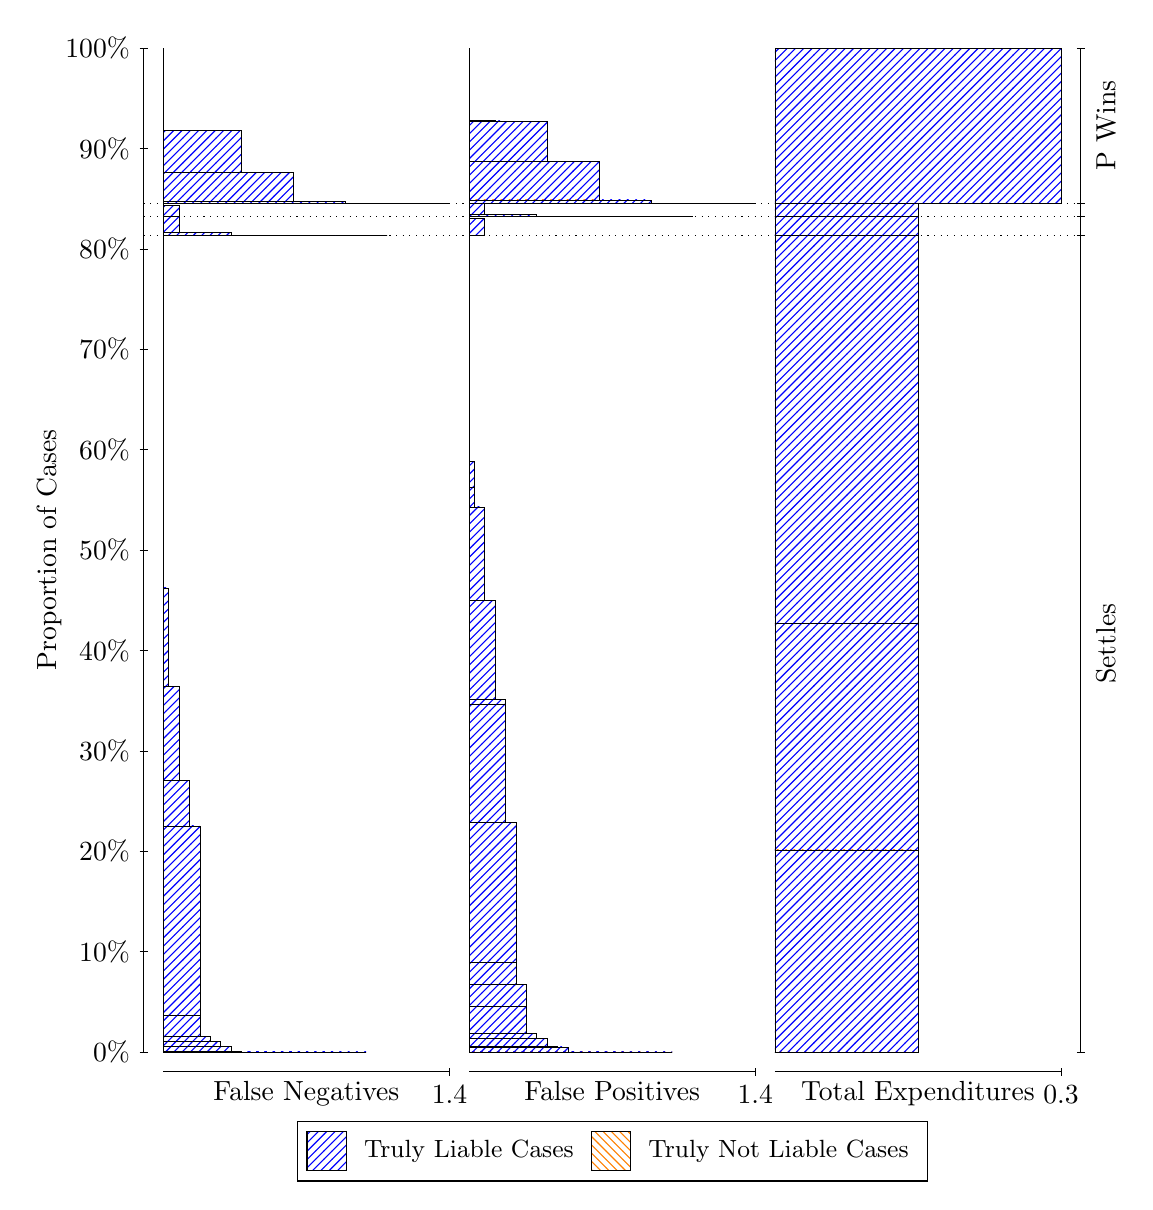
\begin{tikzpicture}
\draw[black, very thin] (1.5,1.75) -- (1.5,14.5);
\node[rotate=90, anchor=center] at (0.3, 8.125) {Proportion of Cases};
\draw[black, very thin] (1.45,1.75) -- (1.55,1.75);
\node[anchor=east] at (1.45, 1.75) {0\%};
\draw[black, very thin] (1.45,3.025) -- (1.55,3.025);
\node[anchor=east] at (1.45, 3.025) {10\%};
\draw[black, very thin] (1.45,4.3) -- (1.55,4.3);
\node[anchor=east] at (1.45, 4.3) {20\%};
\draw[black, very thin] (1.45,5.575) -- (1.55,5.575);
\node[anchor=east] at (1.45, 5.575) {30\%};
\draw[black, very thin] (1.45,6.85) -- (1.55,6.85);
\node[anchor=east] at (1.45, 6.85) {40\%};
\draw[black, very thin] (1.45,8.125) -- (1.55,8.125);
\node[anchor=east] at (1.45, 8.125) {50\%};
\draw[black, very thin] (1.45,9.4) -- (1.55,9.4);
\node[anchor=east] at (1.45, 9.4) {60\%};
\draw[black, very thin] (1.45,10.675) -- (1.55,10.675);
\node[anchor=east] at (1.45, 10.675) {70\%};
\draw[black, very thin] (1.45,11.95) -- (1.55,11.95);
\node[anchor=east] at (1.45, 11.95) {80\%};
\draw[black, very thin] (1.45,13.225) -- (1.55,13.225);
\node[anchor=east] at (1.45, 13.225) {90\%};
\draw[black, very thin] (1.45,14.5) -- (1.55,14.5);
\node[anchor=east] at (1.45, 14.5) {100\%};

\draw[black, very thin] (13.4,1.75) -- (13.4,14.5);
\draw[black, very thin] (13.35,1.75) -- (13.45,1.75);
\node[anchor=west] at (13.35, 1.75) {};
\draw[black, very thin] (13.35,12.122) -- (13.45,12.122);
\node[anchor=west] at (13.35, 12.122) {};
\draw[black, very thin] (13.35,12.366) -- (13.45,12.366);
\node[anchor=west] at (13.35, 12.366) {};
\draw[black, very thin] (13.35,12.531) -- (13.45,12.531);
\node[anchor=west] at (13.35, 12.531) {};
\draw[black, very thin] (13.35,14.5) -- (13.45,14.5);
\node[anchor=west] at (13.35, 14.5) {};

\draw[black, very thin, pattern color=blue, pattern=north east lines] (1.75,1.75) rectangle (4.3264,1.75);
\draw[black, very thin, pattern color=blue, pattern=north east lines] (1.75,1.75) rectangle (4.0621,1.75);
\draw[black, very thin, pattern color=blue, pattern=north east lines] (1.75,1.75) rectangle (3.7979,1.75);
\draw[black, very thin, pattern color=blue, pattern=north east lines] (1.75,1.75) rectangle (3.6658,1.75);
\draw[black, very thin, pattern color=blue, pattern=north east lines] (1.75,1.75) rectangle (3.5336,1.75);
\draw[black, very thin, pattern color=blue, pattern=north east lines] (1.75,1.75) rectangle (3.4015,1.75);
\draw[black, very thin, pattern color=blue, pattern=north east lines] (1.75,1.75) rectangle (3.2694,1.7501);
\draw[black, very thin, pattern color=blue, pattern=north east lines] (1.75,1.7501) rectangle (3.1373,1.7501);
\draw[black, very thin, pattern color=blue, pattern=north east lines] (1.75,1.7501) rectangle (3.0052,1.7501);
\draw[black, very thin, pattern color=blue, pattern=north east lines] (1.75,1.7501) rectangle (2.873,1.7501);
\draw[black, very thin, pattern color=blue, pattern=north east lines] (1.75,1.7501) rectangle (2.873,1.7507);
\draw[black, very thin, pattern color=blue, pattern=north east lines] (1.75,1.7507) rectangle (2.7409,1.755);
\draw[black, very thin, pattern color=blue, pattern=north east lines] (1.75,1.755) rectangle (2.6088,1.8194);
\draw[black, very thin, pattern color=blue, pattern=north east lines] (1.75,1.8194) rectangle (2.4767,1.8847);
\draw[black, very thin, pattern color=blue, pattern=north east lines] (1.75,1.8847) rectangle (2.4767,1.8847);
\draw[black, very thin, pattern color=blue, pattern=north east lines] (1.75,1.8847) rectangle (2.3445,1.9452);
\draw[black, very thin, pattern color=blue, pattern=north east lines] (1.75,1.9452) rectangle (2.2124,1.9452);
\draw[black, very thin, pattern color=blue, pattern=north east lines] (1.75,1.9452) rectangle (2.2124,2.2191);
\draw[black, very thin, pattern color=blue, pattern=north east lines] (1.75,2.2191) rectangle (2.2124,4.6211);
\draw[black, very thin, pattern color=blue, pattern=north east lines] (1.75,4.6211) rectangle (2.0803,5.2);
\draw[black, very thin, pattern color=blue, pattern=north east lines] (1.75,5.2) rectangle (1.9482,6.389);
\draw[black, very thin, pattern color=blue, pattern=north east lines] (1.75,6.389) rectangle (1.8161,7.6444);
\draw[black, very thin, pattern color=blue, pattern=north east lines] (1.75,7.6444) rectangle (1.8161,7.6444);
\draw[black, very thin, pattern color=orange, pattern=north west lines] (1.75,7.6444) rectangle (1.75,7.6444);
\draw[black, very thin, pattern color=blue, pattern=north east lines] (1.75,7.6444) rectangle (1.75,12.122);
\draw[black, very thin, pattern color=blue, pattern=north east lines] (1.75,12.122) rectangle (4.5906,12.122);
\draw[black, very thin, pattern color=blue, pattern=north east lines] (1.75,12.122) rectangle (3.93,12.122);
\draw[black, very thin, pattern color=blue, pattern=north east lines] (1.75,12.122) rectangle (3.2694,12.122);
\draw[black, very thin, pattern color=blue, pattern=north east lines] (1.75,12.122) rectangle (2.6088,12.155);
\draw[black, very thin, pattern color=blue, pattern=north east lines] (1.75,12.155) rectangle (1.9482,12.366);
\draw[black, very thin, pattern color=orange, pattern=north west lines] (1.75,12.366) rectangle (1.75,12.366);
\draw[black, very thin, pattern color=blue, pattern=north east lines] (1.75,12.366) rectangle (1.9482,12.506);
\draw[black, very thin, pattern color=orange, pattern=north west lines] (1.75,12.506) rectangle (1.75,12.506);
\draw[black, very thin, pattern color=blue, pattern=north east lines] (1.75,12.506) rectangle (1.75,12.531);
\draw[black, very thin, pattern color=blue, pattern=north east lines] (1.75,12.531) rectangle (5.3833,12.531);
\draw[black, very thin, pattern color=blue, pattern=north east lines] (1.75,12.531) rectangle (4.7227,12.531);
\draw[black, very thin, pattern color=blue, pattern=north east lines] (1.75,12.531) rectangle (4.0621,12.553);
\draw[black, very thin, pattern color=blue, pattern=north east lines] (1.75,12.553) rectangle (3.5336,12.553);
\draw[black, very thin, pattern color=blue, pattern=north east lines] (1.75,12.553) rectangle (3.4015,12.918);
\draw[black, very thin, pattern color=blue, pattern=north east lines] (1.75,12.918) rectangle (2.873,12.918);
\draw[black, very thin, pattern color=blue, pattern=north east lines] (1.75,12.918) rectangle (2.7409,13.454);
\draw[black, very thin, pattern color=blue, pattern=north east lines] (1.75,13.454) rectangle (2.2124,13.457);
\draw[black, very thin, pattern color=blue, pattern=north east lines] (1.75,13.457) rectangle (2.0803,13.457);
\draw[black, very thin, pattern color=orange, pattern=north west lines] (1.75,13.457) rectangle (1.75,13.457);
\draw[black, very thin, pattern color=blue, pattern=north east lines] (1.75,13.457) rectangle (1.75,14.5);
\draw[black, very thin, pattern color=orange, pattern=north west lines] (5.6333,1.75) rectangle (8.2097,1.75);
\draw[black, very thin, pattern color=blue, pattern=north east lines] (5.6333,1.75) rectangle (8.2097,1.75);
\draw[black, very thin, pattern color=orange, pattern=north west lines] (5.6333,1.75) rectangle (7.9455,1.75);
\draw[black, very thin, pattern color=blue, pattern=north east lines] (5.6333,1.75) rectangle (7.9455,1.75);
\draw[black, very thin, pattern color=orange, pattern=north west lines] (5.6333,1.75) rectangle (7.6812,1.75);
\draw[black, very thin, pattern color=blue, pattern=north east lines] (5.6333,1.75) rectangle (7.6812,1.75);
\draw[black, very thin, pattern color=blue, pattern=north east lines] (5.6333,1.75) rectangle (7.5491,1.75);
\draw[black, very thin, pattern color=orange, pattern=north west lines] (5.6333,1.75) rectangle (7.417,1.75);
\draw[black, very thin, pattern color=blue, pattern=north east lines] (5.6333,1.75) rectangle (7.417,1.75);
\draw[black, very thin, pattern color=blue, pattern=north east lines] (5.6333,1.75) rectangle (7.2848,1.75);
\draw[black, very thin, pattern color=orange, pattern=north west lines] (5.6333,1.75) rectangle (7.1527,1.75);
\draw[black, very thin, pattern color=blue, pattern=north east lines] (5.6333,1.75) rectangle (7.1527,1.7501);
\draw[black, very thin, pattern color=blue, pattern=north east lines] (5.6333,1.7501) rectangle (7.0206,1.7507);
\draw[black, very thin, pattern color=orange, pattern=north west lines] (5.6333,1.7507) rectangle (6.8885,1.7507);
\draw[black, very thin, pattern color=blue, pattern=north east lines] (5.6333,1.7507) rectangle (6.8885,1.7515);
\draw[black, very thin, pattern color=orange, pattern=north west lines] (5.6333,1.7515) rectangle (6.8885,1.7515);
\draw[black, very thin, pattern color=blue, pattern=north east lines] (5.6333,1.7515) rectangle (6.8885,1.8157);
\draw[black, very thin, pattern color=blue, pattern=north east lines] (5.6333,1.8157) rectangle (6.7564,1.8181);
\draw[black, very thin, pattern color=orange, pattern=north west lines] (5.6333,1.8181) rectangle (6.6242,1.8181);
\draw[black, very thin, pattern color=blue, pattern=north east lines] (5.6333,1.8181) rectangle (6.6242,1.9203);
\draw[black, very thin, pattern color=blue, pattern=north east lines] (5.6333,1.9203) rectangle (6.4921,1.9857);
\draw[black, very thin, pattern color=orange, pattern=north west lines] (5.6333,1.9857) rectangle (6.36,1.9857);
\draw[black, very thin, pattern color=blue, pattern=north east lines] (5.6333,1.9857) rectangle (6.36,2.3312);
\draw[black, very thin, pattern color=blue, pattern=north east lines] (5.6333,2.3312) rectangle (6.36,2.6073);
\draw[black, very thin, pattern color=blue, pattern=north east lines] (5.6333,2.6073) rectangle (6.2279,2.8835);
\draw[black, very thin, pattern color=blue, pattern=north east lines] (5.6333,2.8835) rectangle (6.2279,4.6648);
\draw[black, very thin, pattern color=orange, pattern=north west lines] (5.6333,4.6648) rectangle (6.0958,4.6648);
\draw[black, very thin, pattern color=blue, pattern=north east lines] (5.6333,4.6648) rectangle (6.0958,6.1642);
\draw[black, very thin, pattern color=blue, pattern=north east lines] (5.6333,6.1642) rectangle (6.0958,6.2278);
\draw[black, very thin, pattern color=blue, pattern=north east lines] (5.6333,6.2278) rectangle (5.9636,7.4832);
\draw[black, very thin, pattern color=blue, pattern=north east lines] (5.6333,7.4832) rectangle (5.8315,8.6723);
\draw[black, very thin, pattern color=blue, pattern=north east lines] (5.6333,8.6723) rectangle (5.6994,8.9175);
\draw[black, very thin, pattern color=blue, pattern=north east lines] (5.6333,8.9175) rectangle (5.6994,9.2511);
\draw[black, very thin, pattern color=blue, pattern=north east lines] (5.6333,9.2511) rectangle (5.6333,12.122);
\draw[black, very thin, pattern color=orange, pattern=north west lines] (5.6333,12.122) rectangle (5.8315,12.122);
\draw[black, very thin, pattern color=blue, pattern=north east lines] (5.6333,12.122) rectangle (5.8315,12.333);
\draw[black, very thin, pattern color=blue, pattern=north east lines] (5.6333,12.333) rectangle (5.6333,12.366);
\draw[black, very thin, pattern color=orange, pattern=north west lines] (5.6333,12.366) rectangle (8.4739,12.366);
\draw[black, very thin, pattern color=blue, pattern=north east lines] (5.6333,12.366) rectangle (8.4739,12.366);
\draw[black, very thin, pattern color=blue, pattern=north east lines] (5.6333,12.366) rectangle (7.8133,12.366);
\draw[black, very thin, pattern color=blue, pattern=north east lines] (5.6333,12.366) rectangle (7.1527,12.366);
\draw[black, very thin, pattern color=blue, pattern=north east lines] (5.6333,12.366) rectangle (6.4921,12.391);
\draw[black, very thin, pattern color=blue, pattern=north east lines] (5.6333,12.391) rectangle (5.8315,12.531);
\draw[black, very thin, pattern color=orange, pattern=north west lines] (5.6333,12.531) rectangle (9.2667,12.531);
\draw[black, very thin, pattern color=blue, pattern=north east lines] (5.6333,12.531) rectangle (9.2667,12.531);
\draw[black, very thin, pattern color=orange, pattern=north west lines] (5.6333,12.531) rectangle (8.6061,12.531);
\draw[black, very thin, pattern color=blue, pattern=north east lines] (5.6333,12.531) rectangle (8.6061,12.531);
\draw[black, very thin, pattern color=orange, pattern=north west lines] (5.6333,12.531) rectangle (7.9455,12.531);
\draw[black, very thin, pattern color=blue, pattern=north east lines] (5.6333,12.531) rectangle (7.9455,12.571);
\draw[black, very thin, pattern color=orange, pattern=north west lines] (5.6333,12.571) rectangle (7.2848,12.571);
\draw[black, very thin, pattern color=blue, pattern=north east lines] (5.6333,12.571) rectangle (7.2848,13.057);
\draw[black, very thin, pattern color=orange, pattern=north west lines] (5.6333,13.057) rectangle (6.7564,13.057);
\draw[black, very thin, pattern color=blue, pattern=north east lines] (5.6333,13.057) rectangle (6.7564,13.057);
\draw[black, very thin, pattern color=blue, pattern=north east lines] (5.6333,13.057) rectangle (6.6242,13.573);
\draw[black, very thin, pattern color=blue, pattern=north east lines] (5.6333,13.573) rectangle (6.0958,13.573);
\draw[black, very thin, pattern color=orange, pattern=north west lines] (5.6333,13.573) rectangle (6.0958,13.573);
\draw[black, very thin, pattern color=blue, pattern=north east lines] (5.6333,13.573) rectangle (6.0958,13.574);
\draw[black, very thin, pattern color=blue, pattern=north east lines] (5.6333,13.574) rectangle (5.9636,13.577);
\draw[black, very thin, pattern color=orange, pattern=north west lines] (5.6333,13.577) rectangle (5.6333,13.577);
\draw[black, very thin, pattern color=blue, pattern=north east lines] (5.6333,13.577) rectangle (5.6333,14.5);
\draw[black, very thin, pattern color=orange, pattern=north west lines] (9.5167,1.75) rectangle (11.333,1.75);
\draw[black, very thin, pattern color=blue, pattern=north east lines] (9.5167,1.75) rectangle (11.333,4.3156);
\draw[black, very thin, pattern color=orange, pattern=north west lines] (9.5167,4.3156) rectangle (11.333,4.3156);
\draw[black, very thin, pattern color=blue, pattern=north east lines] (9.5167,4.3156) rectangle (11.333,7.1905);
\draw[black, very thin, pattern color=orange, pattern=north west lines] (9.5167,7.1905) rectangle (11.333,7.1905);
\draw[black, very thin, pattern color=blue, pattern=north east lines] (9.5167,7.1905) rectangle (11.333,12.122);
\draw[black, very thin, pattern color=orange, pattern=north west lines] (9.5167,12.122) rectangle (11.333,12.122);
\draw[black, very thin, pattern color=blue, pattern=north east lines] (9.5167,12.122) rectangle (11.333,12.366);
\draw[black, very thin, pattern color=orange, pattern=north west lines] (9.5167,12.366) rectangle (11.333,12.366);
\draw[black, very thin, pattern color=blue, pattern=north east lines] (9.5167,12.366) rectangle (11.333,12.531);
\draw[black, very thin, pattern color=orange, pattern=north west lines] (9.5167,12.531) rectangle (13.15,12.531);
\draw[black, very thin, pattern color=blue, pattern=north east lines] (9.5167,12.531) rectangle (13.15,14.5);
\draw[black, dotted] (1.5,12.122) -- (13.4,12.122);
\draw[black, dotted] (1.5,12.366) -- (13.4,12.366);
\draw[black, dotted] (1.5,12.531) -- (13.4,12.531);
\draw[black, very thin] (1.75,1.5) -- (5.3833,1.5);
\node[anchor=north] at (3.5667, 1.5) {False Negatives};
\draw[black, very thin] (5.3833,1.45) -- (5.3833,1.55);
\node[anchor=north] at (5.3833, 1.45) {1.4};

\draw[black, very thin] (5.6333,1.5) -- (9.2667,1.5);
\node[anchor=north] at (7.45, 1.5) {False Positives};
\draw[black, very thin] (9.2667,1.45) -- (9.2667,1.55);
\node[anchor=north] at (9.2667, 1.45) {1.4};

\draw[black, very thin] (9.5167,1.5) -- (13.15,1.5);
\node[anchor=north] at (11.333, 1.5) {Total Expenditures};
\draw[black, very thin] (13.15,1.45) -- (13.15,1.55);
\node[anchor=north] at (13.15, 1.45) {0.3};

\node[black, centered, rotate=90] at (13.72, 6.9361) {Settles};


\node[black, centered, rotate=90] at (13.72, 13.515) {P Wins};

\draw (7.449999999999999,1.5) node[draw=none] (baseCoordinate) {};
\begin{scope}[align=center]
        \matrix[scale=0.5, draw=black, below=0.5cm of baseCoordinate, nodes={draw}, column sep=0.1cm]{
            \node[rectangle, draw, minimum width=0.5cm, minimum height=0.5cm, pattern=north east lines, pattern color=blue] {}; &
            \node[draw=none, font=\small] (B) {Truly Liable Cases}; &
            \node[rectangle, draw, minimum width=0.5cm, minimum height=0.5cm, pattern=north west lines, pattern color=orange] {}; &
            \node[draw=none, font=\small] (B) {Truly Not Liable Cases}; \\
            };
\end{scope}

\end{tikzpicture}
\end{document}